\documentclass[11pt]{article}
\usepackage[utf8]{inputenc}
\usepackage[spanish]{babel}
\usepackage{epsfig}
\usepackage{fullpage}
\usepackage{graphicx}
\usepackage{rotating}
%\usepackage{pdflscape}
\usepackage{lscape}

\usepackage{verbatim}
\usepackage{algorithm}
\usepackage{algorithmic}

\parskip 2mm
\parindent 0mm

% Comandos latex para imprimir una figura ".eps" centrada
\def\centeredeps#1{\begin{center}\leavevmode\epsfbox{#1.eps}\end{center}}

% Comando para imprimir el encabezado
\def\logo{\mbox{\epsfbox{utalca.eps}}\hspace{1em}\large
 \begin{tabular}[b]{l}
  \sc Universidad de Talca \\
  \sc Facultad de Ingenier\'ia \\
  \sc Ingenier\'ia Civil en Computaci\'on \\
  %\vspace{15\baselineskip}\mbox{}
  \vspace{-5.5mm}\mbox{}
 \end{tabular}
 \normalsize
 \vspace{\baselineskip}
}


\pagestyle{empty}

\begin{document}

\logo

\vspace{-2mm}
\begin{center}
\bf Algoritmos y estructuras de datos\\
\large Informe tarea N$^\circ$ 3\\
\vspace{1mm}
\small\bf 10 de Julio de 2012
\end{center}
\vspace{-2mm}


\section{Introducción}
Él problema principal reside en ordenar elementos alojados en la memoria auxiliar (HDD) utilizando la menor cantidad posible de memoria fisica (RAM), dado que el conjunto de datos a ordenar supera enormemente la cantidad de memoria fisica disponible.

\section{Solucion del problema}
	\subsection{Análisis del problema y algoritmo de solucion}
		Dado los antecedentes anteriores, utilizar algoritmos tipicos de ordenamiento en memoria fisica, tales como \textit{Quicksort}. Pero dado que la memoria auxiliar tambien puede ser utilizada de la misma forma que la fisica, estos algoritmos pueden facilmente ser implementados, pero nos enfrentamos al problema de que la escritura y lectura es lenta.
		
		\begin{algorithm}[H]
		\caption{lectura en disco}
		\label{alg_lecturaDisco}
		\begin{algorithmic}   
			\STATE mover aguja a posicion
			\STATE leer contenido
		\end{algorithmic}
		\end{algorithm}
	
	Pero el leer el contenido de la memoria auxiliar en si es mucho mas lento comparado con una lectua en memoria fisica sea la cantidad de datos que sean, el mover la aguja en si, toma un tiempo constante. Este tiempo constante, si bien no es mucho, ha de ser multiplicado por la cantidad de lecturas que es nesesario realizar para poder cargar la informacion completa. Debido a esto, los algoritmos que no son estables, o que nececitan de muchas operaciones de insercion, intercambio o eliminacion se ven enormenente desfavorecidas.
	
	Una de las formas de lograr ordenar esto, es dividir el archivo en partes que sea posible ordenarlas en la memoria auxiliar, y luego combinar todas estas soluciones para poder obtener el conjunto final de datos, completamente ordenados. El algoritmo de ordenamiento \textit{MergeSort} funciona de esa manera, combinando soluciones en memoria fisica, tomando en cuenta, que los trozos que ha de mezclar ya estan previamente ordenados, lo cual deja el funcionamiento de nuestro programa asi:
	
		\begin{algorithm}[H]
		\caption{$principal(vias)$}
		\label{alg_programaPrincipal}
		\begin{algorithmic}   
			\STATE $generacion \leftarrow 0$
			\STATE $numeroPaginas \leftarrow separarArchivo(tamanoPaginaMemoria)$
			\WHILE {$numeroPaginas > 1$}
				\STATE $numeroPaginas \leftarrow mezclar( generacion, numeroPaginas, vias)$
				\STATE $borrarGeneracion(generacion)$
				\STATE $generacion \leftarrow generacion + 1$
			\ENDWHILE
			\STATE $renombrar(generacion)$
		\end{algorithmic}
		\end{algorithm}
	
	La primera de las subrutinas que se han de implementar es la de la separacion de archivos. Para ese efecto, se procede a leer el archivo binarizado, leyendo de a un dato a la vez, hasta llegar al final del archivo. El resultado de esta lectua es almacenada en un \textit{buffer} de memoria, el cual ha de ser la cantidad de ram objetivo a utlizar. Para efectos de la tarea este numero esta truncado a $2^16 $ ($65536$) bytes (equivalentes a $2^20$ ($1048576$) bits ).\\
	
	Dado esto, el numero de paginas a obtener se puede calcular utlizando la formula:
	
	$$
		numeroPaginas = \lceil\frac{tamanoArchivo}{paginaMemoria}\rceil
	$$
	
	Por lo cual es nesesario tener disponible adicionales en el disco, una cantidad equivalente a el doble de el tamaño del archivo original ya que hasta ahora el tamaño que ha de emplear el algoritmo ha de ser:
	
	$$
		memoriaTotal = memoriaPaginas + memoriaArchivoOriginal
	$$
	
	Una vez lleno este buffer, es volcado hacia la memoria auxiliar, y luego se sigue llenandose secuencialmente. Esto es para darle algo mas de flexibilidad al momento de encontrar conjuntos de datos cuyo tamaño no esten truncados en el tamaño especificado. Dado que se utiliza un heap para administrar el contenido de la pagina, al momento de volcarse esta, se garantiza que los datos esten ordenados.
	
		\begin{algorithm}[H]
		\caption{separarArchivo($tamanoPaginaMemoria$)}
		\label{alg_separacion}
		\begin{algorithmic}   
			\STATE $numeroPaginas \leftarrow 0$
			\STATE $buf \leftarrow new Buffer(tamanoPaginaMemoria)$
			\WHILE {$!archivo.fin()$}
				\STATE $buf.push(archivo.readByte())$
				\IF{$buf.estaLleno()$}
					\STATE $buf.volcar()$
					\STATE $numeroPaginas \leftarrow numeroPaginas +1$
				\ENDIF
			\ENDWHILE
			\RETURN $numeroPaginas$
		\end{algorithmic}
		\end{algorithm}
		
	Luego de ejecutar la separacion del archivo, para poder ordenarlos, dependiendo si es ordenamiento de miltiples vias, o de via doble. Para ello se utiliza un heap, para poder tener un acceso ordenado a los datos. El funcionamiento es relativamente simple asi que no requiere mayor explicacion; para cada uno de los archivos se lee solo un byte. Luego, este byte, es agregado al heap minimo, de modo de obtener el dato menor. Al momento de recibir el dato, se revisa la pagina de donde provino, y se le pide un nuevo dato. Si a esta se le agotan, entonces se llego al fin de la pagina y se omite. Todo el procedimiento anterior termina cuando todas las paginas han sido revisadas (y por ende mezcladas).
		
		\begin{algorithm}[H]
		\caption{mezclar($generacion, numeroPaginas ,vias$)}
		\label{alg_separacion}
		\begin{algorithmic}   
			\STATE $numeroPaginasProsesadas \leftarrow 0$
			\WHILE {$numeroPaginasProsesadas < numeroPaginas$}
				\STATE $mezclarGeneracion(generacion,vias,numeroPaginasProsesadas)$
			\ENDWHILE
			\RETURN $numeroPaginasProsesadas$
		\end{algorithmic}
		\end{algorithm}
		
		\begin{algorithm}[H]
		\caption{mezclarGeneracion($generacion, vias, iteracion)$}
		\label{alg_mezclar}
		\begin{algorithmic}   
			\STATE $administradorPaginas \leftarrow new PageAdmin(generacion, vias, iteracion)$
			\STATE $archivoSalida \leftarrow new ArchivoSalida(generacion+1, iteracion)$
			\WHILE {$!administradorPaginas.hasNext()$}
				\STATE $archivoSalida.push(administradorPaginas.nextInt())$
				\IF{$archivoSalida.estaLleno()$}
					\STATE $archivoSalida.write()$
				\ENDIF
			\ENDWHILE
			\STATE $archivoSalida.write()$
			\STATE $archivoSalida.close()$
		\end{algorithmic}
		\end{algorithm}
						
	
	\subsection{Diagrama de estados}

	  	\begin{figure}[H]
  			\centering
    		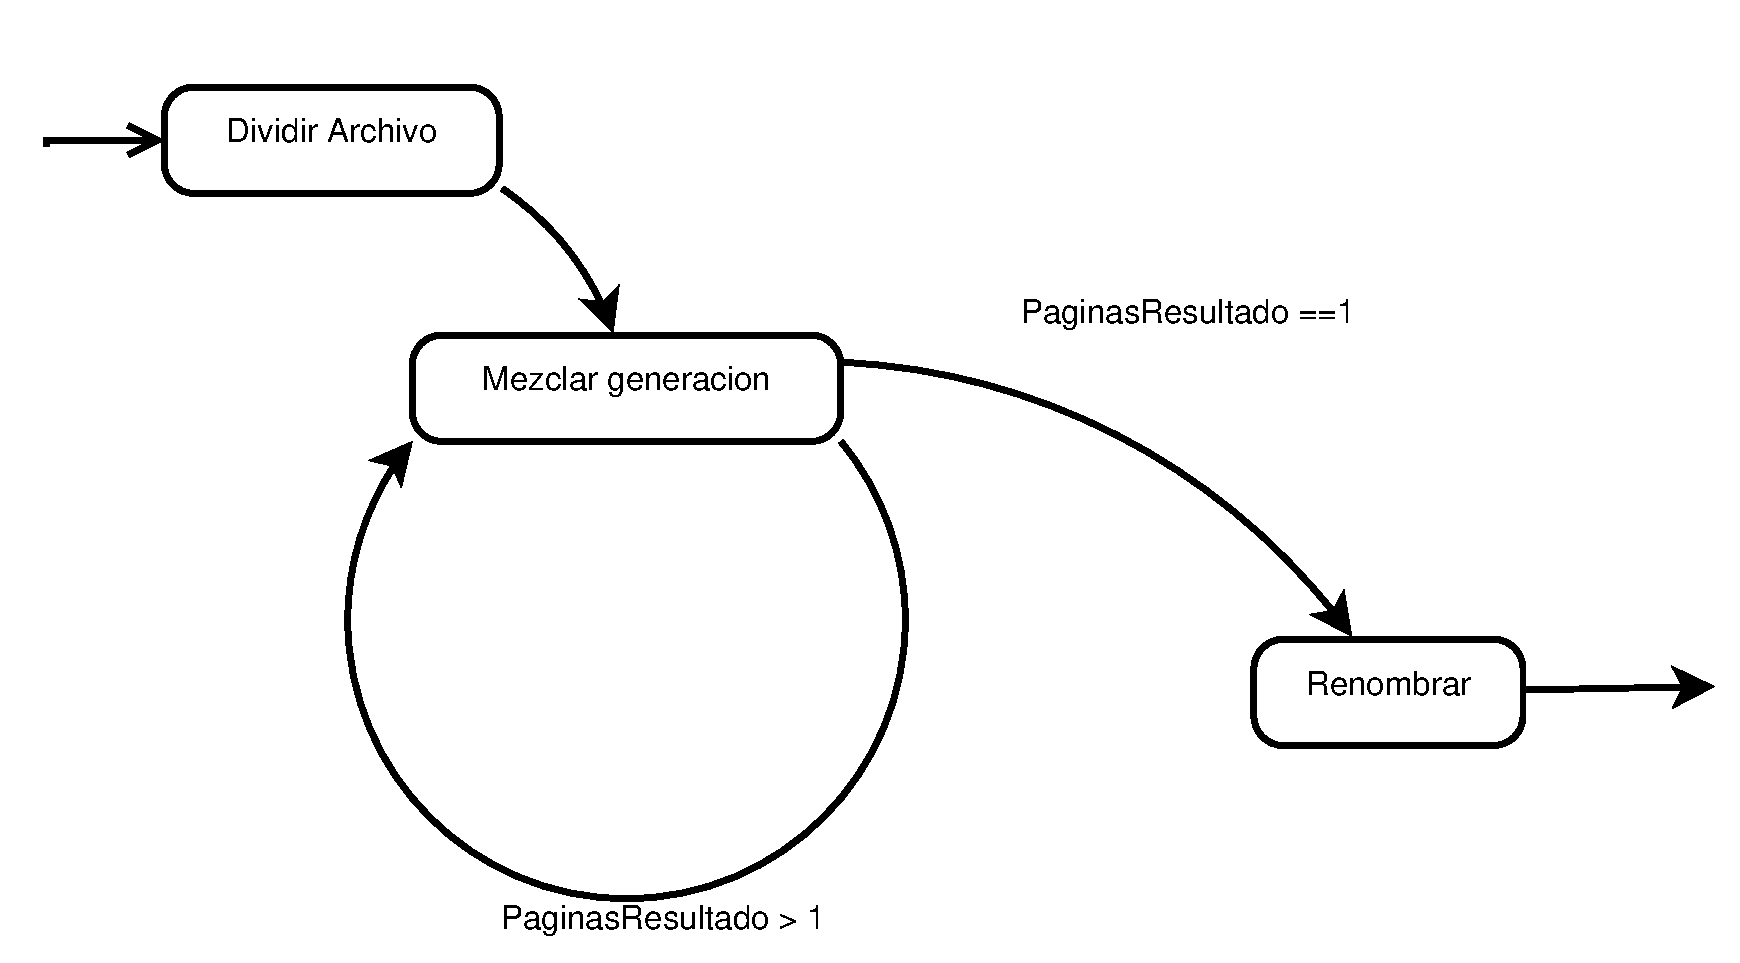
\includegraphics[width=0.85\textwidth]{Diagram3}
  			\caption{Programa principal, primer estado de desorden}
		\end{figure}
		\begin{figure}[H]
  			\centering
    		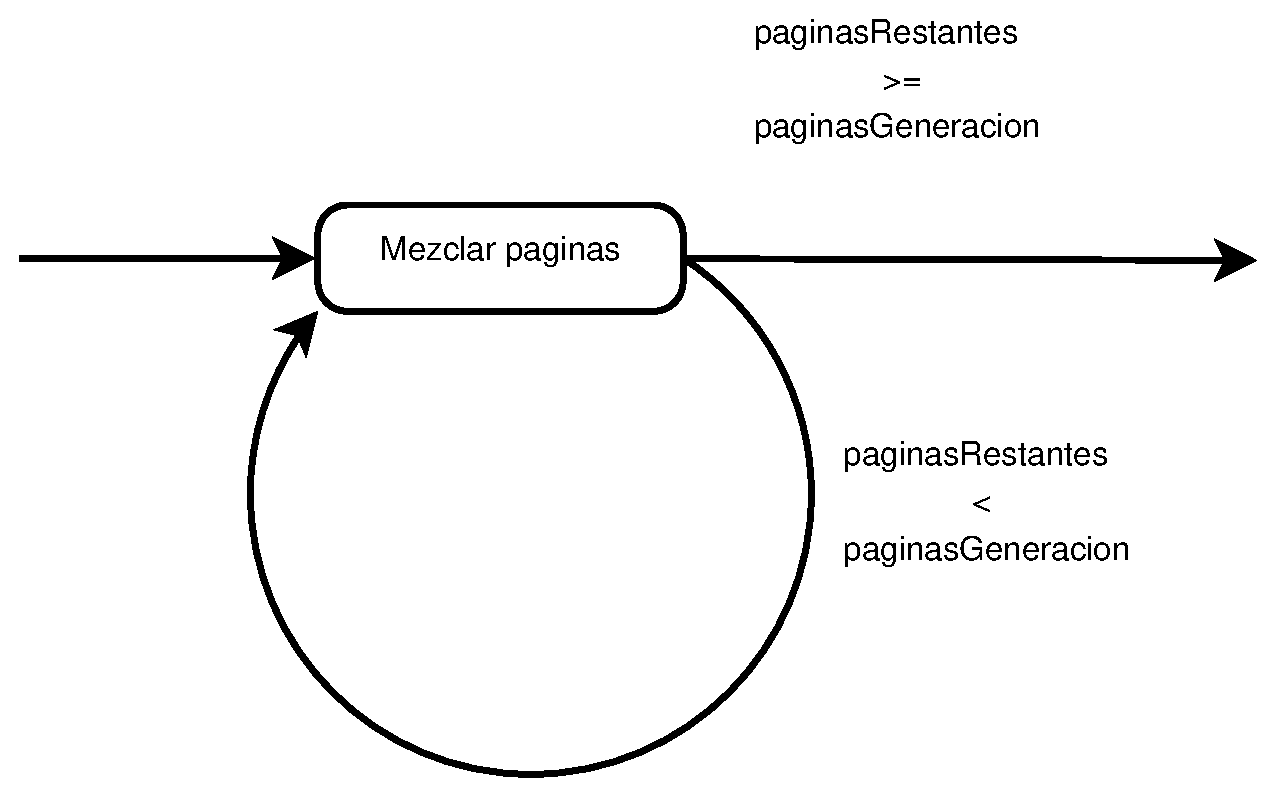
\includegraphics[width=0.85\textwidth]{Diagram2}
  			\caption{Estado de ordenamiento}
		\end{figure}
		\begin{figure}[H]
  			\centering
    		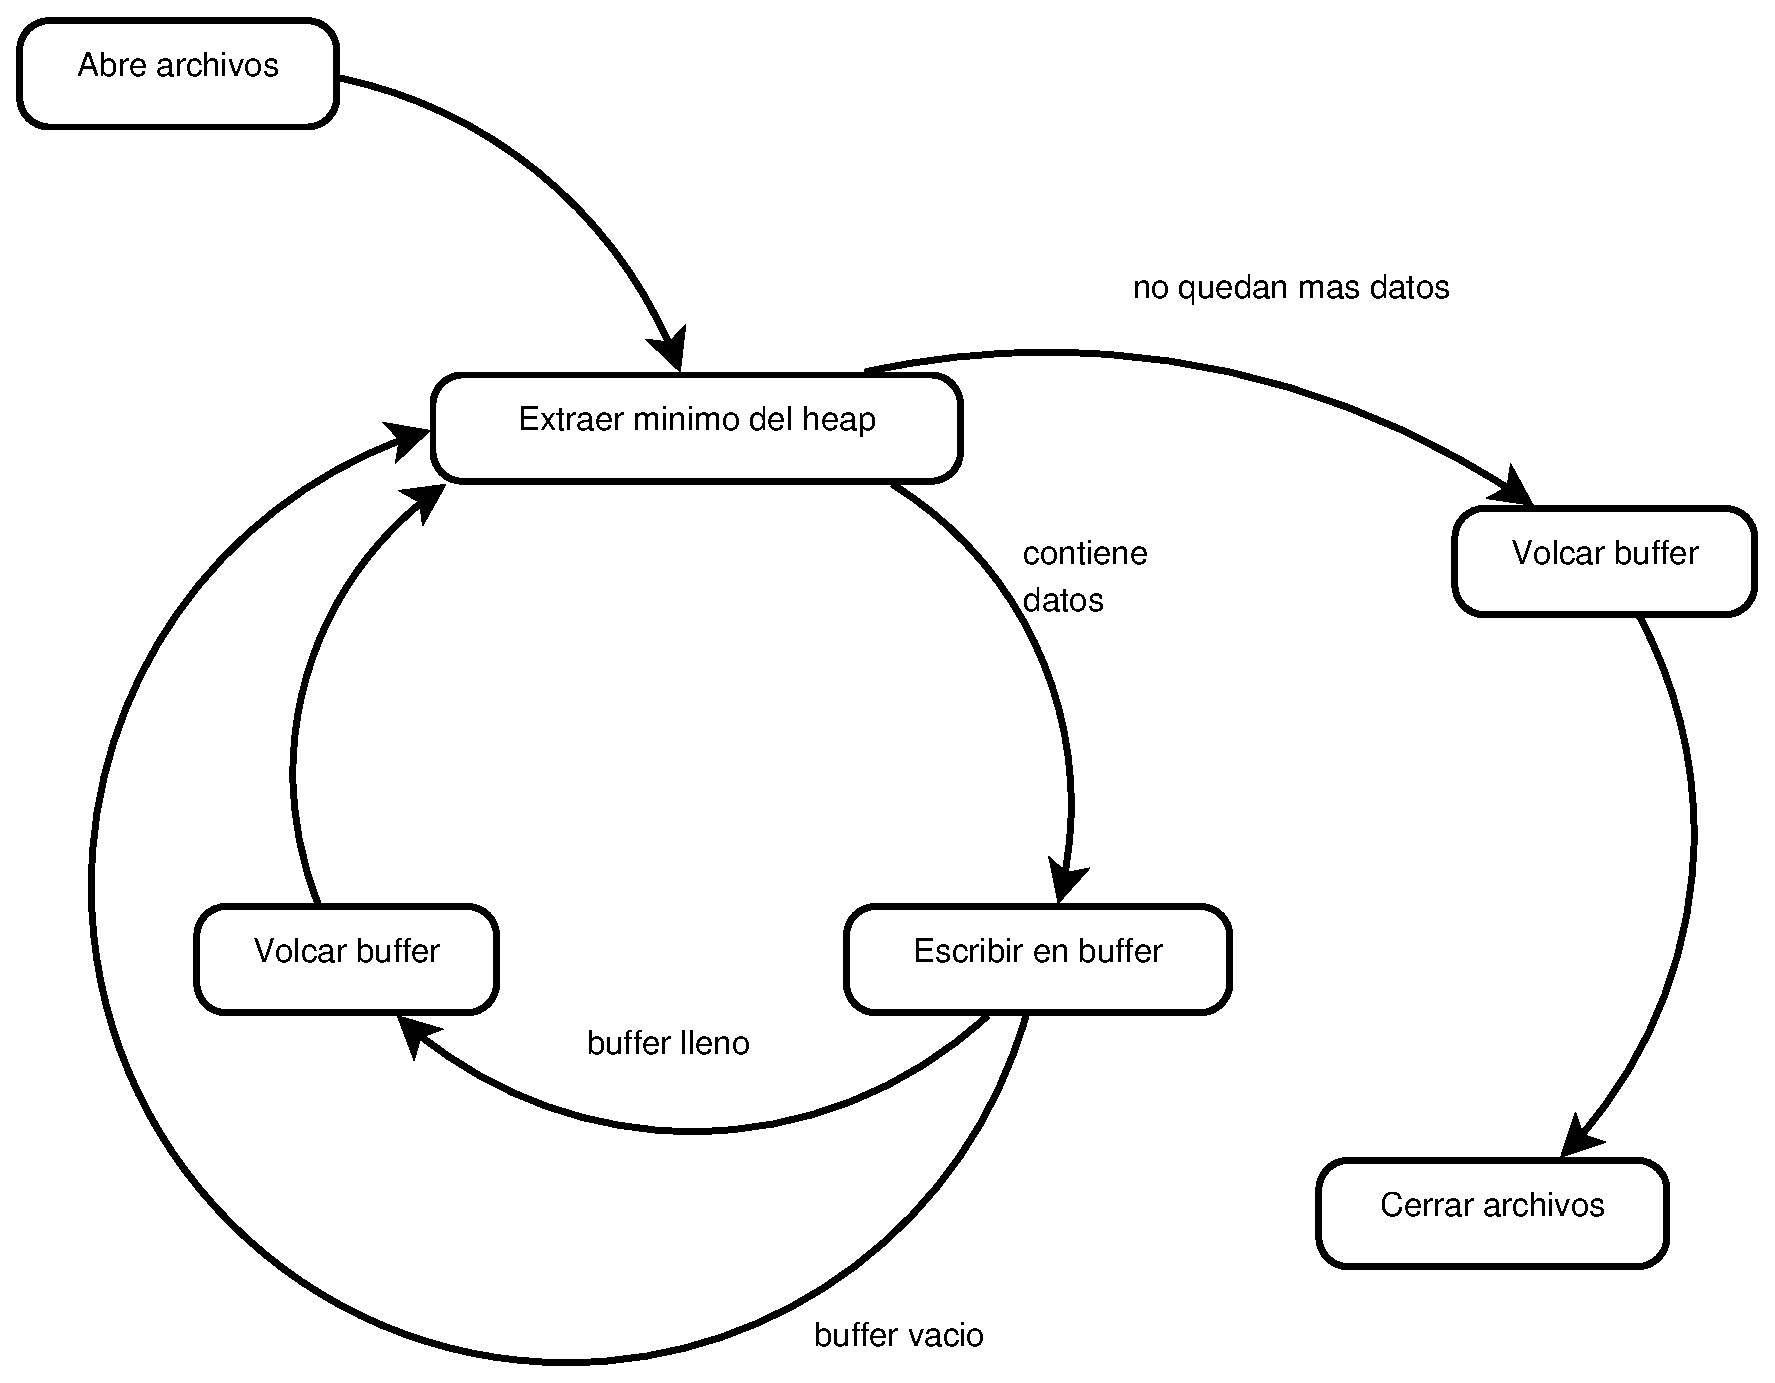
\includegraphics[width=0.85\textwidth]{Diagram1}
  			\caption{Ordenamiento de pagina y mezclado}
		\end{figure}
	
\subsection{Resultados de las pruebas}
Pendiente.

%%agregado a ultima hora, por que parece q la version q subi no tenia eso.. XD
\section{Instalacion y uso del programa}
Dentro del tar se encuentra un espacio de trabajo de eclipse, en el cual hay dos proyectos nombrados  ''proyecto3\_2w" y ``proyecto3\_8w" escritos en el lenguaje C++. Estos contienen el mismo programa en si, el cual ejecuta una version del proyecto diferente -en el codigo se encuentra escrita la diferencia-, uno hecho para ejecutarse bajo dos vias (Mergesort comun) y otro para ejecutarse bajo 8 vias (MultiWay-Mergesort). Para poder compilar el programa, se nececita importar el proyecto a eclipse,y luego ejecutar el comando ``build". Esto deja en el directorio ``Debug" un archivo ejecutable, con el mismo nombre del proyecto compilado. Este ejecutable ha de ser dejado en el directorio en donde se encuentra el archivo ``data.bin", el cual ha de contener el conjunto de numeros desordenados en formato binario. Para dar inicio, basta con solo ejecutar el progama y este comenzara a ordenar solo el archivo en cuestion, y dejara escrito un archivo de nombre ``data.bin\_sorted", el cual contiene el archivo mezclado y ordenado.\\

Nota: El programa fue hecho pensandose que se ejecutara en alguna maquina con un entorno basado en UNIX, como Linux o Mac.

\end{document}














%La Gran Vendimia de Chile versión 2012, es la fiesta del vino más grande de la región del Maule y en la cual participan destacados elaboradores y 
%productores de vino del país. Este año los organizadores del evento decidieron que para la siguiente versión del evento, a realizarse el próximo año, 
%inscribir a los participantes de los stands de manera electrónica, por lo cual necesitan de su ayuda para la implementación de este sistema.
%
%Para la inscripción para tal magno evento cada elaborador o productor deberá proporcionar la siguiente información:
%
%\begin{itemize}
%  \itemsep -2mm
%  \item nombre
%  \item ubicación de la planta (ciudad)
%  \item número de contacto del representante
%  \item email 
%  \item lista de los vinos a presentar
%\end{itemize}
%
%La información de los vinos a insertar corresponde a la siguiente:
%\begin{itemize}
%  \itemsep -2mm
%  \item Nombre del Vino
%  \item Cepa
%  \item Valle
%  \item Precio
%  \item Descripción
%\end{itemize}
%
%Con estos datos en el sistema, los organizadores del evento asignan a cada empresa un stand alrededor de la plaza de Curicó, distribuyéndolos 
%como se puede ver en el siguiente mapa:
%
%\begin{center}
% %\includegraphics[width=220px]{./images/pa_2012-1_lab1_i1.eps}
% % pa_2012-1_lab1_i1.eps: 0x0 pixel, 300dpi, 0.00x0.00 cm, bb=-0 -0 405 335
%\end{center}
% 
%La denominación usada para realizar las asignaciones es Punto Cardinal -- Número, por ejemplo, Viña Miguel Torres se encuentra localizado en Norte-1, 
%Viña Correa Albano se encuentra en Este-2.
%
%Usted está encargado de realizar el sistema que permita la inscripción de cada empresa y su correspondiente asignación de stand. 
%Para ello debe modelar e implementar las clases necesarias para cumplir con su cometido. 
%
%Además debe implementar todos los métodos necesarios para consultar la información de las diferentes empresas y sus vinos, 
%para ello la búsqueda debe realizarse a través de la ubicación del stand. La información a mostrar en cada resultado de búsqueda es la siguiente:
%
%\begin{itemize}
%  \itemsep -1mm
%  \item Nombre de la Viña
%  \item Número de Contacto
%  \item Stand
%  \item Email
%  \item Listado con la información de los vinos.
%\end{itemize}
%